\textit{Cette phase d'analyse est un élément indispensable à la bonne réalisation du projet. Dans un premier temps, un modèle plus fidèle à la réalité des schémas stockés dans les SGBDR est présenté. Cette partie est suivit d'une petite réflexion sur l'utilisation des ORM. Sont ensuite parcourus les solutions de génération de graphes pour la représentation des données. Les choix concernant l'interface utilisateur seront également exposés.}

\section{Le modèle}
\subsection{Modèle réellement rencontré}

Lors de l'étude des métadonnées stockées par les différents SGBD, nous avons remarqué quelque divergences par rapport au modèle fournit avec le sujet (figure~\ref{figure:diag_classe_fournit} page~\pageref{figure:diag_classe_fournit}). La figure~\ref{figure:diag_classe_reel} présente un diagramme de classe construit suite à nos recherches.

\begin{figure}[H]
\centering
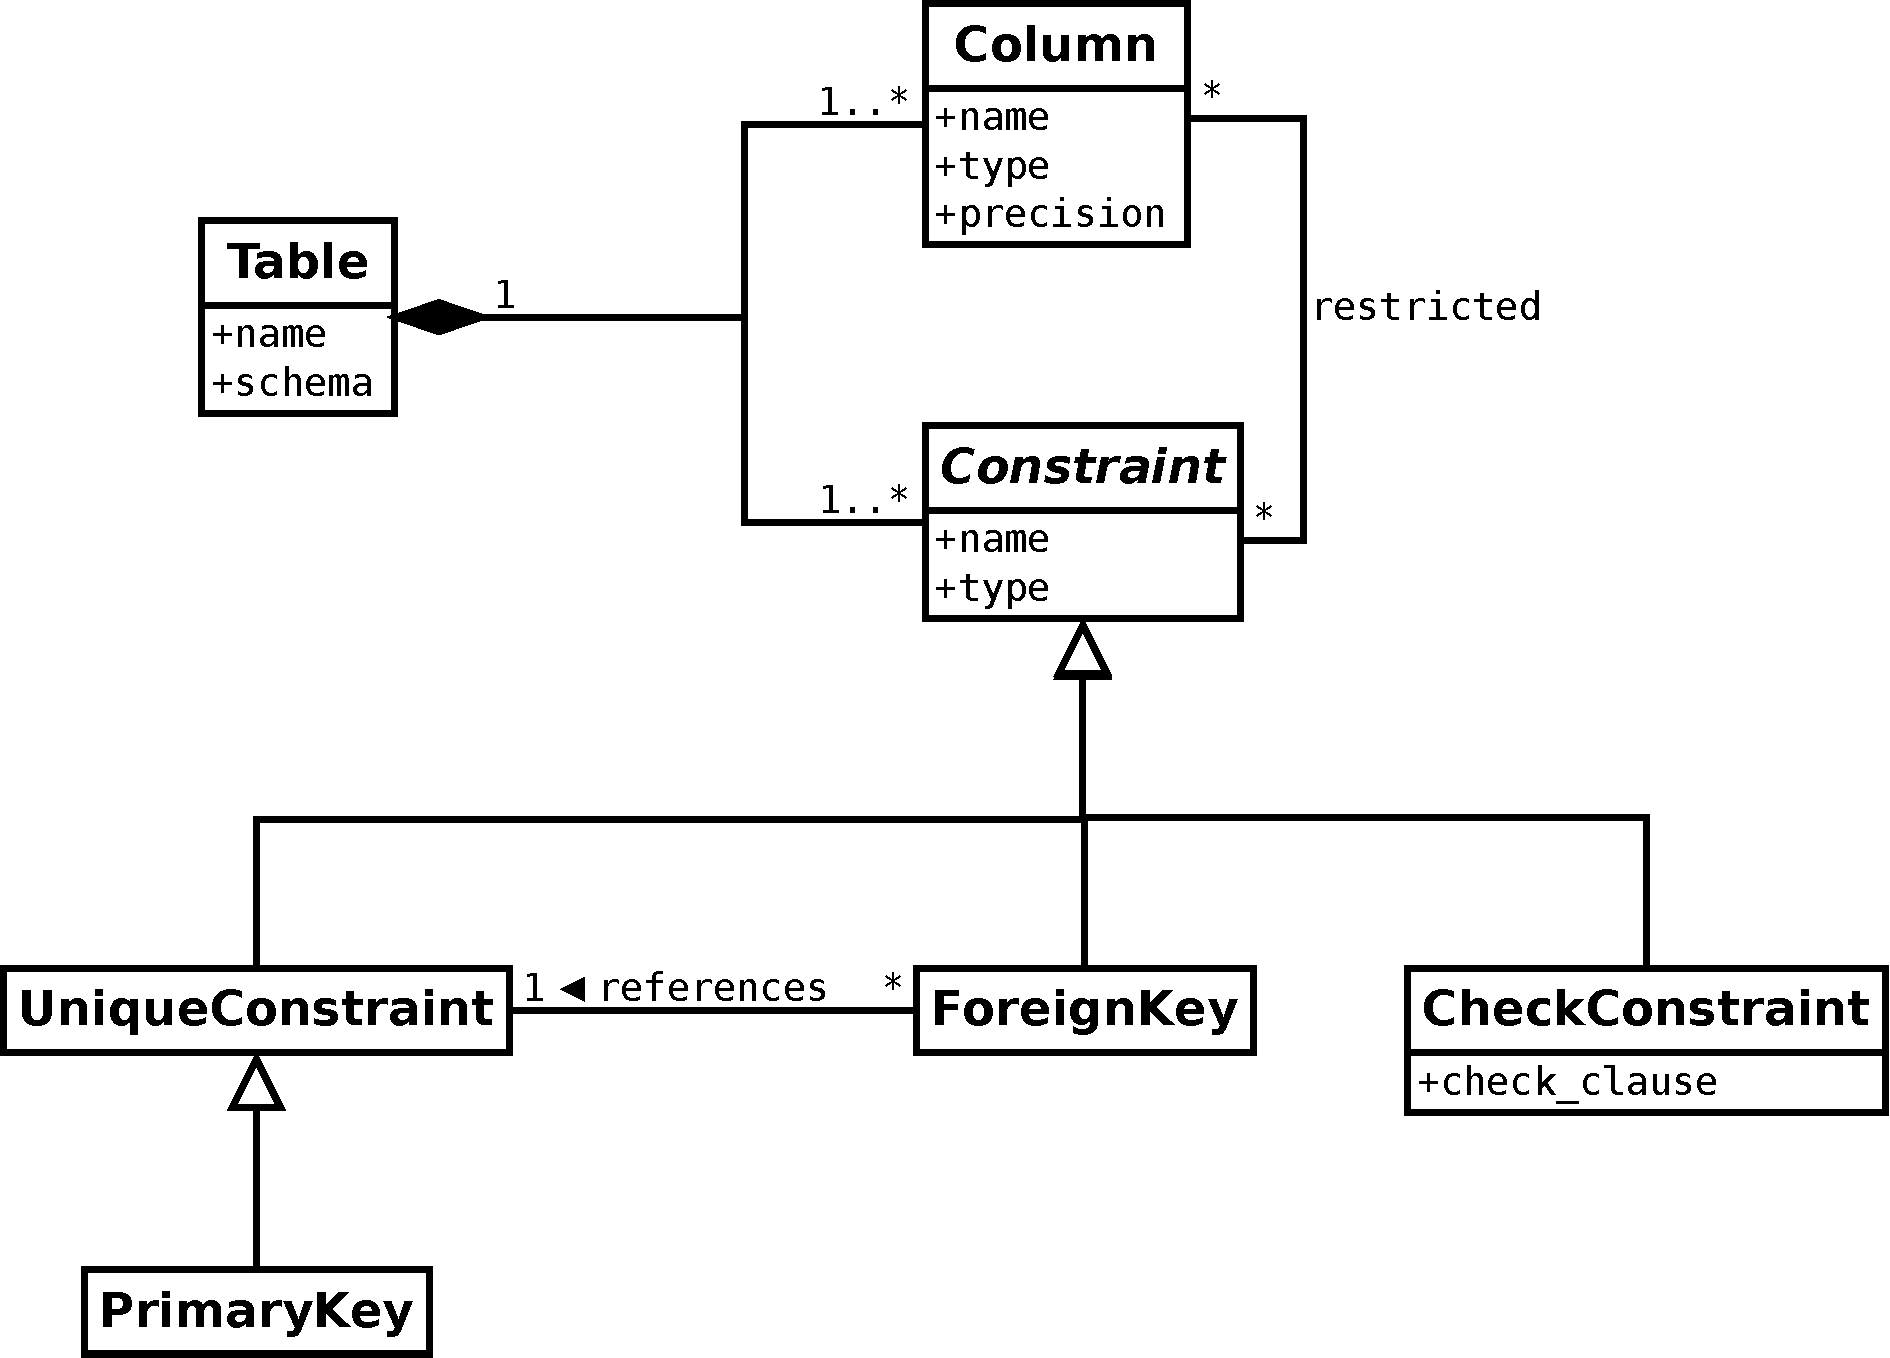
\includegraphics[width=\textwidth]{files/diag_class_ameliore}
\caption{Diagramme de classe réellement rencontré.}
\label{figure:diag_classe_reel}
\end{figure}

La principale différence réside dans la classification des contraintes. Cette classification permet de distinguer trois types de contraintes :

\begin{itemize}
\item Les contraintes d'unicité : elles contraignent l'unicité d'un ou plusieurs attributs au sein d'une même table. Les contraintes de clé primaire sont des contraintes d'unicité.
\item Les contraintes d'intégrité référentielle : elles identifient un ou plusieurs attributs d'une table comme référençant un ou plusieurs attributs d'une autre table, au travers d'une contrainte d'unicité. Notons que ce type de contrainte permet de \textbf{référencer une contrainte d'unicité et non plus une contrainte de clé primaire} comme proposé dans le modèle original.
\item Les contraintes de type \emph{Check} : qui s'appliquent à un ou plusieurs attributs d'une table. Elles contiennent une clause de vérification \texttt{check\_clause}.
\end{itemize}

\paragraph*{NB}
Les contraintes de type \emph{NULL}, \emph{NOT NULL} et \emph{DEFAULT} sont ignorées.

	\subsection{Tables}
		Une table est identifiée par son nom et le schéma auquel elle appartient. Elle possède un ensemble de colonnes et un ensemble de contraintes.
	\subsection{Colonne}
		Une colonne est identifiée par son nom et la table à laquelle elle appartient. Elle possède un type, et éventuellement une précision. 
	\subsection{Contraintes}
		Une contrainte est identifié par un nom, sur certain SGBD il faut lui adjoindre le nom de la table sur laquelle elle est appliquée pour avoir une identification unique (notamment MySQL). Une contrainte possède un type et s'applique sur une ou plusieurs colonne d'une table. Elle peut être de type \og primary key \fg{}, \og foreign key \fg{}, \og unique \fg{} ou \og check \fg. Les contraintes de type \og foreign key \fg{} référence en plus une contrainte de type unique compatible, c'est à dire que les colonnes sur lesquelles s'applique la \og foreign key \fg{} et les colonnes sur lesquelles s'applique la contrainte référencée sont au même nombres et de même types. 
\section{ORM}

	\subsection{Qu'est qu'un ORM?}
    Un ORM ou \emph{mapping objet-relationnel} (en anglais \emph{object-relational mapping}) est une méthode de programmation qui consiste à donner l'illusion d'une base de données orientée objet à partir d'une base de données relationnelle en implémentant une interface entre celle-ci et le code de l'application. Il permet donc de palier aux problèmes d'adaptation entre le paradigme objet et les SGBDR en remplaçant les accès à la base de données par des appels à des méthodes objet de haut niveau.
   
	\subsection{Pourquoi?}
    Les systèmes de gestion de bases de données orientées objet étant actuellement peu nombreux et la norme SQL3 étant que partiellement implémentée, les ORM offre à ce jour le meilleur compromis entre la performance des SGBDR et le pouvoir expressif de la modélisation objet.
    
En revanche, cette méthode d'abstraction présente l'inconvénient de générer un schéma différent de la vision objet avec laquelle est modélisée l'application. Il peut parfois être nécessaire d'intervenir directement sur la base de données (développement de TRIGGERS, dump SQL, \ldots), ce qui nécessite alors un effort d'analyse et de compréhension.

\section{Compatibilité avec les SGBD}

	\subsection{Gestion des types génériques}
	\label{section:generic_types}


\section{Visualisation de graphes}
  \subsection{différentes librairies}
		\paragraph{JUNG} Java Universal Network/Graph Framework\\
				JUNG est une API java permettant la modélisation, l'analyse et la visualisation de graphes. C'est un logiciel libre sous licence BSD\footnote{http://jung.sourceforge.net/license.txt} développé par l'université de Californie.
				inconvénients : dernières fonctionnalités dot non prise en charqe.
		\paragraph{Grappa} A Java \texttt{gra}ph \texttt{pa}ckage\\
			Grappa est une API java de visualisation et manipulation de graphes. C'est un logiciel libre sous CPL\footnote{CPL, Common Public Licence} développé par John Mocenigo d'AT\&T.
				 entrée : fichier dot
		\paragraph{graphviz} Graph Visualization Software\\
			GraphViz est un logiciel de visualisation de graphes écrit en C. C'est un logiciel libre sous EPL\footnote{EPL, Eclipse Public Licence} développé par AT\&T et les laboratoirs Bell. Il offre différents algorithmes de spatialisation. Il est à l'origine du langage de description de graphe \og DOT \fg{}. Il offre une interface en ligne de commande\footnote{man graphviz}.
				
  \subsection{Notre choix}
		\verb+//Notre choix c'est porté sur la commande DOT fournit par GraphViz+

\section{L'IHM}	
	\subsection{les choix possibles}
	\label{ihm_choix_possibles}
		Concernant la conception de l'interface utilisateur, deux choix principaux s'offrent à nous. Le premier est de concevoir
une interface graphique proposant une fenêtre de configuration puis un affichage du résultat obtenu. Le second est de concevoir 	une interface en ligne de commande générant une image. 	
	
		\subsubsection{GUI : \og Graphical User Interface \fg{}}
			Une interface utilisateur graphique permet une prise en main rapide et intuitive d'un logiciel mais ne permet pas une grande interopérabilité. En effet, il est compliqué de demandé à un programme de configurer un autre programme via une interface graphique.
			
		\subsubsection{CLI : \og Command Line Interface \fg{}}
			La conception d'une interface en ligne de commande entre dans la philosophie KISS, « Keep it simple, Stupid! ». Cette philosophie préconise la recherche de simplicité dans la conception et insiste sur le fait que toute complexité non nécessaire devrait être évitée. Cette vision à l'avantage d'offrir une grande interopérabilité, il est en effet aisé d'exécuter une ligne de commande depuis un logiciel et d'en récupérer la sortie. Par contre, une interface en ligne de commande est plus difficile à prendre en main pour un utilisateur non averti.  
			
	\subsection{Notre choix}
		Nous avons choisi pour notre logiciel, d'implémenter une interface en ligne de commande pour les avantages de cette vision, détaillés précédement en \ref{ihm_choix_possibles}, à savoir sa simplicité et sa grande interopérabilité. De plus, nous pouvons, à partir d'une interface en ligne de commande, créer une interface graphique dans un langage quelconque qui encapsule notre logiciel, alors que l'inverse est bien entendu beaucoup moins évident.

